\chapter*{ВВЕДЕНИЕ}							% Заголовок
\addcontentsline{toc}{chapter}{ВВЕДЕНИЕ}	% Добавляем его в оглавление

В настоящее время набрала большую популярность передача поддержки ИТ-инфраструктуры предприятия во внешнюю компанию \cite{StartToOutsource}. Явление это стало называться «ИТ-Аутсорсинг» (от анг. "out source" \- вне источника). В некоторых случаях это дает возможность экономии до 30\% по данным Gartner \cite{OutsourceIT}. Ввиду развития рынка компаниям становится невыгодно держать свой штат службы поддержки, и они отдают ее сторонней компании \cite{OutsourceEff}. В некоторых случаях передается вся поддержка пользователей: будь то сломанный компьютер или же простое не знание внутренних процессов компании. То есть создается единая точка входа для пользователей, поддерживаемая сторонней компанией \cite{OutsourceSD}. (Обобщая можно сказать, что на аутсорсинг передают все, что возможно: управление персоналом, уборка, кейтеринг, разработка ПО \cite{OutsourceSoft} и т.д. \\
Из-за возросшей популярности данного бизнеса и появления большого количества игроков на рынке возникла большая конкуренция \cite{AUTOS-1}, что потребовало увеличения эффективности и сокращения издержек, что в свою очередь привело к необходимости системного анализа области и выработке решения сложившихся проблем \cite{AUTOM-1} ввиду падения рентабильности бизнеса как минимум для малых компаний \cite{OUTSOURCE-RENT} \cite{OutsourceEff}. В контексте этой проблемы рассматривается модель области и модель системы, которая увеличивает эффективность работы путем частичной (в некоторых случаях полной) автоматизации обработки инцидентов \cite{SDAUTOM}, начиная с разбора на естественном языке и заканчивая применением найденного решения. \\
Главным требованием к подобной системе является замена части функций, которые сейчас обеспечивают специалисты:
\begin{enumerate}
  \item Обработка запросов на естественном языке. Данная функция широко востребована в системах анализа проблем пользователя с построением отчета успешности того или иного программного продукта \cite{TUTUB-1}
  \item Возможность обучения. Данная возможность системы позволяет упростит ее эксплуатацию и расширение. По данным исследования \cite{LEARN-1} возможность обучения систем является высоковостребованной.
  \item Общение с человеческим специалистом. Поддержание диалога (коммуникации) необходимое условие для обучения. Кроме того социальная функция неотъемлемая часть интеллектуальных систем \cite{LEARN-2}
  \item Проведение логических рассуждений: аналогия, дедукция, индукция. Умение абстрагировать решение одной проблемы и, экстраполируя его, применить для других решений. Данное понятие также обозначается термином "Принятие решений". Например, это широко используется в интеллектуальных системах управления производством \cite{LEARN-3}
\end{enumerate}

На данный момент компании ведут разработку подобных систем. Примером является набирающая популярность IBM Watson \cite{WATSON-PO} \cite{WATSON-PTOP}. Подобный класс систем также называется вопросно-ответными системами. Однако, система является коммерческой и закрытой, информации о ее внутреннем устройстве мало. В рамках исследования \cite{TUTUB-2} была решена задача автоматического определения проблем из отчетов пользователей о пользовании программным обеспечением.\\
В данной работе была произведена попытка создания подобной системы на основе исследования целевой области (удаленная поддержка информационной структуры предприятия) и построения ее модели.
 Акцент был сделан на создании интеллектуальной системы для решения широкого круга проблем. \\
Большинство проблем, которые решает удаленная служба поддержки носят весьма тривиальный характер (по данным компании ОАО ICL-КПО ВС).
\begin{itemize}
	\item Установить приложение
	\item Переустановить приложение
	\item Решить проблему с доступом к тому или иному ресурсу
\end{itemize}
Данные проблемы решают специалисты технической поддержки. Обычно техническая поддержка делится на несколько линий по уровню умения специалистов.

\begin{table} [htbp]
  \centering
  \parbox{15cm}{\caption{Описание работы специалистов различных уровней поддержки}\label{TSSDescription}}
%  \begin{center}
  \begin{tabular}{| p{7cm} || p{7cm} |}
  \hline
  \hline
Уровень & Описание \\
  \hline
    \hline

Первая линия	& Решение уже известных, задокументированных проблем, работа напрямую с пользователем \\
  \hline

Вторая линия  & Решение ранее неизвестных проблем \\
  \hline

Третья линия & Решение сложных и нетривиальных проблем \\
  \hline

Четвертая линия  & Решение архитектурных проблем инфраструктуры \\

  \hline
  \hline
  \end{tabular}
%  \end{center}
\end{table}


Каждая линия поддержки представлена специалистами. В среднем команда, обслуживающая одного заказчика насчитывает 60 человек. Процентное соотношение специалистов разных линий поддержки отображено на Диаграмме \ref{img:ITSMTeamComposition}

\begin{figure} [h] 
  \center
  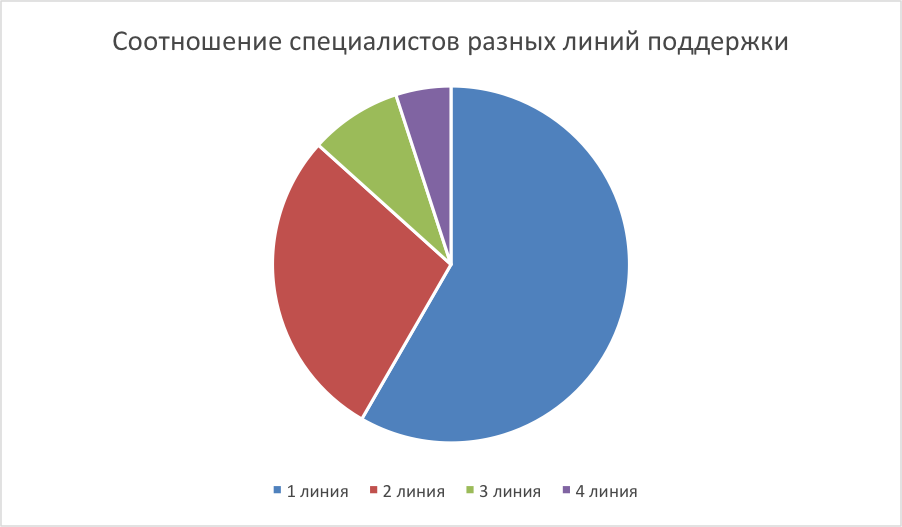
\includegraphics [scale=0.7] {ITSMTeamComposition}
  \caption{Диаграмма состава команд} 
  \label{img:ITSMTeamComposition}  
\end{figure}

Работа специалиста 1 линии поддержки состоит из множества рутинных и простых задач. На Диаграмме \ref{img:EngineerTasks}  показано соотношение разных типов проблем, встречающихся во время работы поддержки

\begin{figure} [h] 
  \center
  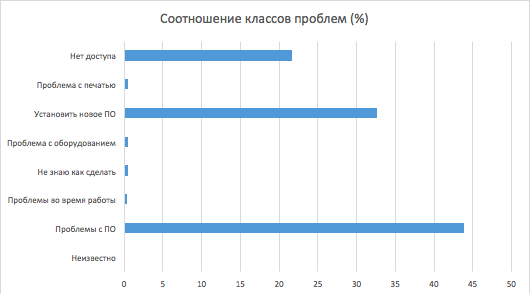
\includegraphics [scale=0.7] {EngineerTasks}
  \caption{Диаграмма соотношений типов проблем} 
  \label{img:EngineerTasks}  
\end{figure}

\begin{table} [htbp]
  \centering
  \parbox{15cm}{\caption{Категории инцидентов в области удаленной поддержки инфраструктуры}\label{IncidentDescription}}
%  \begin{center}
  \begin{tabular}{| p{7cm} || p{7cm} |}
  \hline
  \hline
Категория & Описание \\
  \hline
Проблема с ПО	& Проблема при запуске ПО на компьютере. Решается переустановкой \\
Проблемы во время работы  & Проблема с функционированием программного обеспечения\\
Как сделать & Запрос на инструкцию по работе с тем или иным компонентом рабочей станции \\
Проблема с оборудованием  & Неполадки на уровне оборудования \\
Установить новое ПО       & Требование установки нового программного обеспечения \\
Проблема с печатью        & Установка принтера в систему \\
Нет доступа               & Нет доступа к общим ресурсам \\
  \hline
  \hline
  \end{tabular}
%  \end{center}
\end{table}

Решение части задач может быть автоматизировано, а специалисты получат дополнительное время на решение более интересных задач. 
Проблема заключается в автоматизации решения рутинных задач в области удаленной поддержки инфраструктуры.

%\newpage
%============================================================================================================================

\textbf{Прогноз развития области} 
Основной тенденцией в развитии области удаленной поддержки инфраструктуры является попытки удешевить и улучшить стоимость предоставления услуг \cite{OutsourceEff}. \\
Компании, работающие на этом рынке вкладывают большие деньги в автоматизацию. Кроме того современное развитие науки и техники, а точнее вычислительных мощностей позволяет автоматизацию даже самых наукоемких процессов. \\
Дальнейшим развитием области является замена человеческих специалистов на автоматические системы. Многие ведущие компании ведут разработки в этом направлении. Например, компания HP. Данная компания имеет свою системы по регистрации подобных инцидентов и сейчас ведется работа над автоматизацией системы. \\

\textbf{Методологии, используемые в области IT аутсорсинга: ITIL и ITSM} 
В области IT аутсорсинга есть несколько готовых стандартов ведения работ. Одним из таких стандартов является библиотека ITIL. Данные стандарт описывает лучшие практики организации работ в области IT аутсорсинга. Используемый в библиотеки подход соответствует стандартам ISO 9000 (ГОСТ Р ИСО 9000) .
Наличие стандартов в области диктует унифицированность постановки проблем, а также унифицированность алгоритмов решения. Такие предпосылки говорят о возможности частично или в некоторых случаях полной автоматизации решения проблем. \\
\textbf{Рассчет стоимости работы специалиста при автоматизации} 
По данным аналитики портала SuperJob \cite{SuperJob} средняя зарплата системного администратора с опытом работы в среднем по Казани составляет 30000-35000р за 2014 года. Из расчета на 1 час с учетом 21 рабочих дней в месяце - 179-208 рублей в час. Расход компании на человека складывается по следующий формуле \cite{FiscalCodecs} :
\[
L = R + R*(F_1 +F_2+F_3),
\]
где R выплата человеку в час, F1 НДФЛ 13\%, F2 совокупность отчислений в ФБ 6\%, ПФР 14\%, ТФОМС 2\%, ФФОМС 1,1\%, ФСС 2,9\% , F3 Налог на прибыль 20\%. 
Таким образом, расходы компании на сотрудника варьируются от 285 до 314 в час. Таким образом за 8 часовой рабочий день от 2280 до 2512. Стоимость аренды выделенного сервера (Xeon X3, 1.7 GHz, 8GB RAM, 256GB SSD) стоит 8 900 руб./мес \cite{TimeWeb}. Таким образом за 1 час стоит 53 рубля с учетом 8 часового рабочего дня. Но сервер может работать 24 часа в сутки за исключением простоев на обслуживание, которые составляют не более 5 \%. Итого сервер работает 478,8 часов в месяц. С этой точки зрения сервер будет стоить 18,5 рублей в час. Один сервер в своем быстродействие может заменить несколько специалистов при решении задач. Чтобы решение было экономически эффективном необходимо, чтобы оно сокращало расходы как минимум на 30\%. Грубый подсчет на основе стоимости часа и пропорции показывает, что работа специалиста это 6\% работы сервера (без учета работы сервера как несколько специалистов и примерно одинаковой скорости решения инцидентов). Таким образом уровень решения инцидентов системой в 50\% выполнит требования по прибыли примерно 1027 \%. 


\textbf{Общая характеристика работы} 

\newcommand{\aim}{\textbf{Целью}}
\newcommand{\scope}{\textbf{Область исследования}}
\newcommand{\subject}{\textbf{Предметом исследования}}
 процесс регистрации и устранения проблемных ситуаций, возникающих в IT-инфраструктуре предприятия 
\newcommand{\tasks}{задачи}
\newcommand{\defpositions}{\textbf{Основные положения, выносимые на~защиту:}}
\newcommand{\novelty}{\textbf{Научная новизна:}}
\newcommand{\influence}{\textbf{Практическая значимость}}
\newcommand{\reliability}{\textbf{Степень достоверности}}
\newcommand{\probation}{\textbf{Апробация работы.}}
\newcommand{\contribution}{\textbf{Личный вклад.}}
\newcommand{\publications}{\textbf{Публикации.}}

{\aim} работы является разработка интеллектуальной системы повышения эффективности деятельности ИТ-службы предприятия. \par
{\scope}~--- разработка методов и алгоритмов решения задач системного анализа, оптимизации, управления, принятия решений и обработки информации в ИТ-отрасли.\par
{\subject}  является процесс регистрации и устранения проблемных ситуаций, возникающих в ИТ-инфраструктуре предприятия.\par

Для достижения поставленной цели необходимо было решить следующие {\tasks}:
\begin{enumerate}
  \item Провести теоретико-множественный и теоретико-информационный анализ сложных систем в области поддержки информационной инфраструктуры;
  \item Создать модель целевой области;
  \item Исследовать модели мышления и выбрать наиболее подходящую;
  \item На основе выбранной модели мышления разработать модель проблемно-ориентированной системы управления, принятия решений и оптимизации процесса принятия, анализа и обработки запросов пользователя в области обслуживания информационной структуры предприятия;
  \item Создать архитектуру приложения на основе модели;
  \item Реализовать на основе этой архитектуры прототип интеллектуальной вопросно-ответной системы повышения эффективности деятельности ИТ-службы предприятия;
  \item Провести апробацию прототипа на тестовых данных.
\end{enumerate}

\defpositions
\begin{enumerate}
  \item Теоретико-множественный и теоретико-информационный анализ сложных систем в области поддержки информационной инфраструктуры;
  \item Построенная модель проблемно-ориентированной системы управления, принятия решений и оптимизации технических объектов в области обслуживания информационной инфраструктуры;
  \item Созданный прототип программной реализации модели проблемно-ориентированной системы управления, принятия решений и оптимизации обработки запросов пользователя в области обслуживания информационной инфраструктуры;
  \item Апробация прототипа проблемно-ориентированной системы управления, принятия решений и оптимизации деятельности на контрольных примерах и анализ ее результатов.
\end{enumerate}

\novelty проведенного исследования состоит в следующем:
\begin{enumerate}
  \item Создана модель проблемно-ориентированной системы управления, принятия решений в области обслуживания информационной структуры предприятия на основе модели мышления;
  \item Представлены новая модель данных для модели мышления и оригинальный способ хранения для этой модели, эффективный по сравнению с другими базами данных;
  \item Выполнено оригинальное исследование моделей мышления применительно к области обслуживания информационной структуры предприятия;
  \item На основе модели мышления Мински созданы архитектура системы обслуживания информационной структуры предприятия и программный прототип этой системы.
\end{enumerate}

\influence\ 
Система, разработанная в рамках данной диссертации носит значимый практический характер. Идея работы зародилась под влиянием производственных проблем в ИТ-отрасли, с которыми автор сталкивался каждый день в процессе разрешения различных инцидентов, возникающих в деятельности службы технической поддержки \icl~--- одном из крупнейших системообразующих предприятий ИТ-области Республике Татарстан. Поэтому было необходимо выработать глубокое понимание конкретной предметной области, чтобы выбрать приемлемое решение, получившее практическое применение в работе на проекте поддержки крупной сети продуктовых магазинов. \par
\reliability\ научных исследований и практических рекомендаций
базируется на корректной постановке общих и частных рассматриваемых задач,  использовании известных фундаментальных теоретических положений системного анализа, достаточном объёме данных, использованных при статистическом моделировании, и широком экспериментальном материале, использованном для численных оценок достижимых качественных показателей. \par 
Исследования, проведенные в диссертации, соответствуют паспорту специальности 05.13.01~--- Системный анализ, управление и обработка информации, сопоставление приведено в таблице \ref{ResearchDescription}.

\begin{longtable}{|p{7cm}|p{9cm}|}
 \caption[Сопоставление направлений исследований в рамках специальности 05.13.01 и исследований, проведенных в диссертации]{Сопоставление направлений исследований в рамках специальности 05.13.01 и исследований, проведенных в диссертации}\label{ResearchDescription} \\ 
 \hline
 
 \multicolumn{1}{|c|}{\textbf{Направление исследования}} & \multicolumn{1}{c|}{\textbf{Результат работы}}  \\ \hline 
\endfirsthead
\multicolumn{2}{c}%
{{\bfseries \tablename\ \thetable{} -- продолжение}} \\
\hline \multicolumn{1}{|c|}{\textbf{Направление исследования}} &
\multicolumn{1}{c|}{\textbf{Результат работы}}  \\ \hline 
\endhead

\hline \multicolumn{2}{|r|}{{Продолжение следует}} \\ \hline
\endfoot

\hline \hline
\endlastfoot
\hline
   Разработка критериев и моделей описания и оценки эффективности решения задач системного анализа, оптимизации, управления, принятия решений и обработки информации & В рамках работы была разработана модель системы принятия решения и обработки информации в области решения запросов пользователя на естественном языке. \\
   \hline
   Разработка проблемно-ориентированных систем управления, принятия решений и оптимизации технических объектов & По модели, разработанной в предыдущем пункте был разработан прототип системы принятия решения Thinking Understanding, который был испытан на модельных данных.\\
   \hline
   Методы получения, анализа и обработки экспертной информации & В рамках системы TU был разработан метод обработки экспертной информации - обучение при помощи модели мышления TU, основанной на принципах модели 6-ти Марвина Мински. \\
   \hline
   Разработка специального математического и алгоритмического обеспечения систем анализа, оптимизации, управления, принятия решений и обработки информации & В рамках разработки системы TU были созданы специальные алгоритмы для анализа запросов пользователя и принятия решений.\\
  \hline 
  Теоретико-множественный и теоретико-информационный анализ сложных систем & В рамках работы был проведен комплексный анализ области поддержки программного обеспечения, с помощью которого была построена система данной области и выделены участки для оптимизации принятия решений.\\
  \hline
  Методы и алгоритмы интеллектуальной поддержки при принятии управленческих решений в технических системах & Система, разработанная в рамках данной работы в включает в себя инновационные методы и алгоритмы поддержки принятия решений, использующих в своей основе модель мышления на базе модели мышления Человека, описанной в книге Марвина Мински. \\ 
  \hline
  Визуализация, трансформация и анализ информации на основе компьютерных методов обработки информации & Представлена наглядная визуализация данных по системному анализу области удаленной поддержки инфраструктуры. \\
  \hline	
\end{longtable}


\probation\
 Основные результаты диссертационной работы докладывались на следующих конференциях:
\begin{itemize}
	\item Десятая молодежная научная школа-конференция "Лобачевские чтения~---2011. Казань, 31 октября~--4 ноября 2011";
	\item 3rd World Conference on Information Technology (WCIT-2012); 
	\item Искусственный интеллект и естественный язык (AINL-2013);
	\item Электронная Казань~--- 2014;
	\item Электронные библиотеки: перспективные методы и технологии, электронные коллекции (RCDL-2014);
	\item Agents and multi-agent systems: technologies and applications (AMSTA-2015).
\end{itemize}
Практическая апробация результатов работы проводилась на выгрузке инцидентов из системы регистрации запросов службы технической поддержки ИТ-инфраструктуры \icl. Созданная система показала требуемые результаты (процент успешно обработанных запросов более чем 30\%) обработки данной информации.
\contribution\ Автор исследовал целевую область: проводил анализ запросов пользователей и классифицировал их, вместе с Талановым Максимом Олеговичем изучал модель мышления Марвина Мински; создавал базовую архитектуру систему; вместе с Талановым Максимом Олеговичем проводил разработку компонентов модели, адаптируя теорию Марвина Мински. Автор проводил испытание системы на целевых запросах; отлаживал работу системы.
\publications\ Основные результаты по теме диссертации изложены в 9 печатных изданиях  \cite{Lobachevskii},\cite{WCIT-2012},\cite{AINL-2013},\cite{ISGZ}, \cite{IJSE-1}, \cite{IJSE-2}, \cite{RCDL-2014}, \cite{AMSTA-2015}, \cite{VAK-1}, из которых статьи \cite{RCDL-2014},\cite{AMSTA-2015} проиндексированы в БД Scopus, статья \cite{AMSTA-2015} проиндексирована в БД Web Of Science, работа \cite{VAK-1} опубликована в журнале из списка ВАК, статья  \cite{ISGZ} проиндексирована в БД РИНЦ, работы \cite{Lobachevskii},\cite{WCIT-2012},\cite{AINL-2013},\cite{ISGZ} опубликованы в материалах международных и всероссийских конференций.



 % Характеристика работы по структуре во введении и в автореферате не отличается (ГОСТ Р 7.0.11, пункты 5.3.1 и 9.2.1), потому её загружаем из одного и того же внешнего файла, предварительно задав форму выделения некоторым параметрам
%% регистрируем счётчики в системе totcounter
\regtotcounter{totalcount@figure}
\regtotcounter{totalcount@table}       % Если поставить в преамбуле то ошибка в числе таблиц
\regtotcounter{TotPages}               % Если поставить в преамбуле то ошибка в числе страниц

\textbf{Объем и структура работы.} Диссертация состоит из введения, четырех глав, заключения и пяти приложений. Полный объём диссертации составляет \formbytotal{TotPages}{страниц}{у}{ы}{} 
с~\formbytotal{totalcount@figure}{рисунк}{ом}{ами}{ами}
и~\formbytotal{totalcount@table}{таблиц}{ей}{ами}{ами}. Список литературы содержит  
\formbytotal{citenum}{наименован}{ие}{ия}{ий}.
\clearpage



  \begin{longtable}{| p{5cm} |p{10cm} |}
 \caption[Словарь терминов]{Словарь терминов}\label{Glossary} \\ 
 \hline
 
 \multicolumn{1}{|c|}{\textbf{Термин}} & \multicolumn{1}{c|}{\textbf{Значение}}  \\ \hline 
\endfirsthead
\multicolumn{2}{c}%
{{\bfseries \tablename\ \thetable{} -- продолжение}} \\
\hline \multicolumn{1}{|c|}{\textbf{Термин}} &
\multicolumn{1}{c|}{\textbf{Значение}}  \\ \hline 
\endhead

\hline \multicolumn{2}{|r|}{{Продолжение следует}} \\ \hline
\endfoot

\hline \hline
\endlastfoot
\hline
База Знаний	& База данных приложения, представленная в виде онтологии знаний \\
 \hline
WayToThink	& Путь мышления. Основан на определении Марвина Мински \cite{EmotionMachine}. Класс объектов, которые модифицируют данные \\
 \hline
Critic	& Критик. Основан на определении Марвина Мински \cite{EmotionMachine}. Класс объектов, которые выступают триггерами при наступление определенного события \\
 \hline
ThinkingLifeCycle	& TLC. Основан на определении Марвина Мински \cite{EmotionMachine}. Класс объектов, которые выступают основными объектами для запуска в приложении - рабочими процессами \\
 \hline
Selector	& Компонент, отвечающий за выборку данных из Базы Знаний \\
\hline
Instinctive	& Инстинктивный уровень \\
\hline
Learned	& Уровень обученных реакций \\
\hline
Deliberative	& Уровень рассуждений \\
\hline
Reflective	& Рефлексивный уровень \\
\hline
Self-Reflective Thinking	 & Саморефлексивный уровень \\
\hline
Self-Conscious Reflection	& Самосознательный уровень \\
\hline
ThinkingUnderstanding	& Система, созданная в рамках работы. Дословный перевод "Мышление-Понимание".  \\
\hline
TU	& Сокращение от ThinkingUnderstanding.  \\
\hline
\end{longtable}

\clearpage

\begin{longtable}{|p{7cm}|p{8cm}|}
 \caption[Принятые аннотации для изложения]{Принятые аннотации для изложения}\label{AnnotationsList} \\ 
 \hline
 
 \multicolumn{1}{|c|}{\textbf{Аннотация}} & \multicolumn{1}{c|}{\textbf{Описание}}  \\ \hline 
\endfirsthead
\multicolumn{2}{c}%
{{\bfseries \tablename\ \thetable{} -- продолжение}} \\
\hline \multicolumn{1}{|c|}{\textbf{Аннотация}} &
\multicolumn{1}{c|}{\textbf{Описание}}  \\ \hline 
\endhead

\hline \multicolumn{2}{|r|}{{Продолжение следует}} \\ \hline
\endfoot

\hline \hline
\endlastfoot
\hline
   selectLinkedObject(obj:Resource, linkName:String): Link<Resource>  & Описание метода. selectLinkedObject - название метода. (obj:Resource, linkName:String) - параметры метода. linkName - имя параметра. String тип данных. Link<Resource> - тип возвращаемых данных. Если метод данных не возвращает, то ничего не указывается.\\
   \hline
    \end{longtable}
\clearpage